%----------------------------------------------------------------------------------------
%	PACKAGES AND THEMES
%----------------------------------------------------------------------------------------

\documentclass[serif]{beamer}

% allows the pdf to open in presentation mode immediately on open
\hypersetup{pdfpagemode=FullScreen}
\mode<presentation> {

% The Beamer class comes with a number of default slide themes
% which change the colors and layouts of slides. Below this is a list
% of all the themes, uncomment each in turn to see what they look like.

%\usetheme{default}      % plain
%\usetheme{AnnArbor}    % pretty good (yellow with blue accents)
%\usetheme{Antibes}      % deep blue, brief info at top
%\usetheme{Bergen}       % cornell note style, blue side bar takes up too much room
%\usetheme{Berkeley}     % brief info in blue side bar, shrinks available slide space
%\usetheme{Berlin}       % deep blue, brief now at bottom, shrinks slide space
\usetheme{Boadilla}     % very light blue colors, popped text blocks, close to plain
%\usetheme{CambridgeUS}      % dark reds and light grays
%\usetheme{Copenhagen}       % dark blue, names highlighted @ bottom in black
%\usetheme{Darmstadt}        % Copenhagen theme, minus bottom brief, black accent bar @ top
%\usetheme{Dresden}          % names blue, above short title purple, purple accents
%\usetheme{Frankfurt}        % Copenhagen with popped blocks
%\usetheme{Goettingen}       % brief info in gray side bar on right, plain otherwise
%\usetheme{Hannover}         % Geottingen but bar is on left and skinnier
%\usetheme{Ilmenau}          % Dreden, makes slide space smaller
%\usetheme{JuanLesPins}      % Copenhagen, but no names, short title in black bar at top, shrinks slides 
%\usetheme{Luebeck}          % sharp angles, blue short title, black names
%\usetheme{Madrid}           % blue, purple names, blue short title, light blue date, all at bottom 
%\usetheme{Malmoe}           % no title banners, names black, short title blue @ bottom
%\usetheme{Marburg}          % brief info in black -> blue gradient sidebar on right, shrinks slide
%\usetheme{Montpellier}      % short title in white banner at top, too plain
%\usetheme{PaloAlto}         % Large blue title banner + left side blue banner for brief info
%\usetheme{Pittsburgh}       % titles aligned right, no banners top or bottom
%\usetheme{Rochester}        % Large blue title banners on all 
%\usetheme{Singapore}        % Gradient blue title banner, otherwise plain
%\usetheme{Szeged}           % Striped title banner, stripe separating brief info @ bottom
%\usetheme{Warsaw}           % blue -> black (left -> right) title banner, names black, shorttile blue 

% As well as themes, the Beamer class has a number of color themes
% for any slide theme. Uncomment each of these in turn to see how it
% changes the colors of your current slide theme.

%\usecolortheme{albatross}       % blue backgrounds
%\usecolortheme{beaver}          % hightlights titles in grey blocks, red accents
%\usecolortheme{beetle}          % grey backgrounds
%\usecolortheme{crane}           % highlights titles in yellow blocks
%\usecolortheme{dolphin}         % blue accents, relatively plain
%\usecolortheme{dove}            % only black text
%\usecolortheme{fly}             % all grey slides
%\usecolortheme{lily}            % blocks of text not colored
\usecolortheme{orchid}          % blocks of texted colors darker
%\usecolortheme{rose}            % very light colors on text blocks
%\usecolortheme{seagull}         % grey blocks of text
%\usecolortheme{seahorse}        % steel colored text blocks
%\usecolortheme{whale}           % blues become darker, blue title banners
%\usecolortheme{wolverine}       % yellow title bars with blue accents

%\setbeamertemplate{footline} % To remove the footer line in all slides uncomment this line
%\setbeamertemplate{footline}[fg, page number] % To replace the footer line in all slides with a simple slide count uncomment this line
%\setbeamertemplate{footline}[page number, \insertshorttitle{}]
\setbeamertemplate{navigation symbols}{} % To remove the navigation symbols from the bottom of all slides uncomment this line
}   % end \mode<presentation>

\usepackage{graphicx} % Allows including images
\usepackage{booktabs} % Allows the use of \toprule, \midrule and \bottomrule in tables
\usepackage{animate}
\usepackage{subcaption}
\usepackage{tikz, pgfplots}
    \pgfplotsset{compat=1.15}
\usepackage{amsmath}
\usepackage{multicol}
% videos
\usepackage{multimedia}

% commands
\renewcommand{\vec}[1]{\mathbf{#1}}
\newcommand{\tr}[1]{\mathrm{tr}\left(#1\right)}
\newcommand{\norm}[1]{\left|\left| #1 \right|\right|}
\newcommand{\inner}[1]{\left\langle #1 \right\rangle}
\newcommand{\R}{\mathbb{R}}
\renewcommand{\exp}[1]{\mathrm{exp}\left( #1 \right)}

% page setup
%\everymath{\displaystyle}


% derivatives
\newcommand{\der}[3][1]{
	\frac{{\text{d}^{
		\ifthenelse{\equal{#1}{1}}{}{\,#1}
	}
	{#2} }}
	{\text{d} {#3}^{
		\ifthenelse{\equal{#1}{1}}{}{#1}
	}
	}
}

\newcommand{\pder}[3][1]{
	\frac{\partial^{
		\ifthenelse{\equal{#1}{1}}{}{\,#1}
	}
	{#2}}
	{\partial {#3}^{
		\ifthenelse{\equal{#1}{1}}{}{#1}
	}
	}
}

\everymath{\displaystyle}


\def\sigmacr{\sigma_{\mathrm{crit}}}
\def\E{\mathbb{E}}
\def\V{\mathbb{V}}

%	TITLE PAGE

\title[Horrible Problems]{How to Solve Your Horrible Equation using FEniCS} 

\author{Jerome Troy}

\institute[UD]{University of Delaware}

\date{April 29, 2020} % Date, can be changed to a custom date


% ----------------------------------------------------------------------------------------
% begin the actual presentation
\begin{document}

% title slide
\begin{frame}
\titlepage % Print the title page as the first slide
\end{frame}

\begin{frame}{What is FEniCS?}
    \begin{itemize}
        \item Finite Element Computational Software
        \item Gives intuitive implementations for the finite element method to solve PDEs
        \item Written in Python - easy to understand 
        \item Mirrors mathematical notation
        \item Github for codes used: \url{https://github.com/JeromeTroy/fenics-hgss.git}
    \end{itemize}
    
    \centering
    
\includegraphics[scale=0.25]{figures/fenics-logo.png}
\end{frame}


\begin{frame}{A Brief Introduction to Finite Elements}
    \begin{itemize}
        \item How it works:
        
        \[
            Lu = f, \quad \text{some boundary conditions}
        \]
        
        \item Discretize domain, $\Omega$, into some mesh
        
        \item Choose a \textit{Test function} $v$ such that $v = 0$ on the (Diriclet part of) boundary
        
        \[
            \int_\Omega v Lu \, dx = \int_\Omega v f \, dx
        \]
        
        \item Integrate by parts, boundary condition on $v$ makes 
        boundary terms vanish
        \item Reduces order of derivatives in equation through integration
        
        \item FEniCS wraps functional analysis parts of finite elements nicely so they are all taken care of
    \end{itemize}
\end{frame}


\begin{frame}{An Example}
    \begin{itemize}
    \item Consider Laplace's Equation in a Circle of radius 1, with Dirichlet 
    Boundary Condition:
    
    \begin{equation}
        \label{eq:laplace-dirichlet-circle}
        \begin{split}
            \nabla^2 u = \partial_x^2 u + \partial_y^2 u = f(\vec x), \quad &  
            \vec x \in \Omega := \left\{\vec x \in \R^2 : 0 \leq \norm{\vec x} 
            < 1\right\} \\
            & u(\vec x \in \partial \Omega) = 1
        \end{split}
    \end{equation}

    \item Let $v$ be a piecewise $C^1(\Omega)$ test function such that 
    $v(\vec x) = 0 \quad \forall \vec x \in \partial \Omega$
    
    \item Variational form
    
    \[\begin{split}
        \int_\Omega v \nabla^2 u \, d\vec x = 
        \int_{\partial \Omega} v \pder{u}{n} \, d\sigma - 
        \int_\Omega \nabla v \cdot \nabla u \, d\vec x = 
        \int_\Omega v f(\vec x) \, d\vec x
    \end{split}\]
    
    \[
        \text{BC on} \, v \implies A(u, v) := -\int_\Omega \nabla v \cdot \nabla u \, d \vec x = 
        \int_\Omega v f(\vec x) \, d\vec x =: F(v; f)
    \]
    \end{itemize}
\end{frame}

\begin{frame}{The Code}
    \centering
    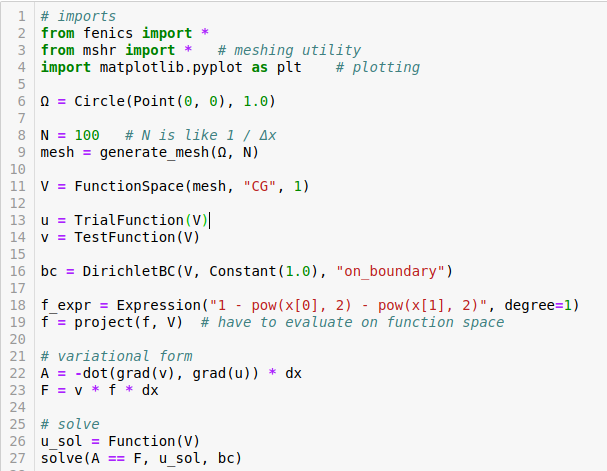
\includegraphics[width=0.9\textwidth,height=0.9\textheight,keepaspectratio]
    {code-snippets/jupyter-fencis-laplace-circle.png}
\end{frame}

\begin{frame}{Solution using FEniCS}

    Example: $f(\vec x) = 1 - \norm{\vec x}^2_2$
    \centering
    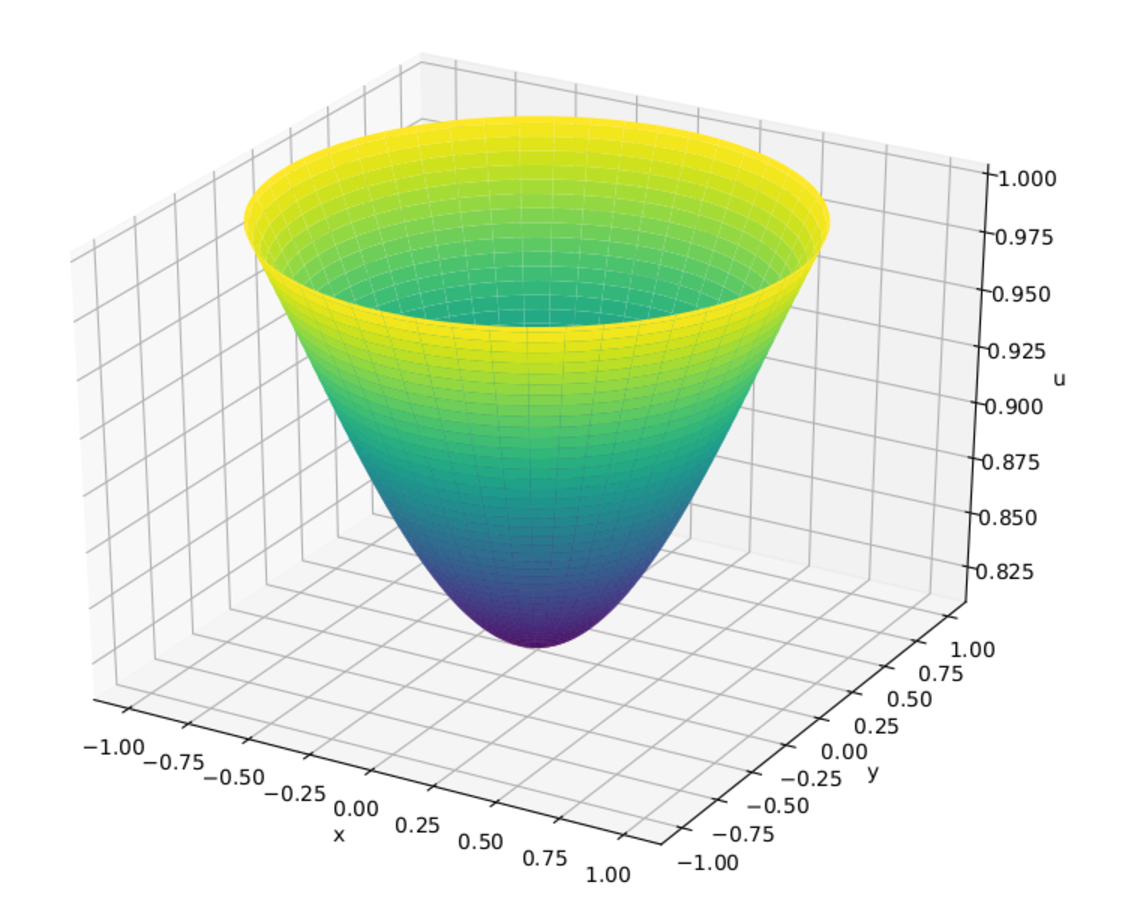
\includegraphics[height=0.75\textheight]{figures/fenics-laplace-circle.pdf}
    
    Norm-2 Error: 0.002392
    
\end{frame}


\begin{frame}{A Time Dependent Example}
    \begin{itemize}
        \item Consider the heat equation:
        
        \begin{equation}
            \label{eq:heat-dirichlet-circle}
            \begin{split}
            \pder{u}{t} = \nabla \cdot (\kappa \nabla u), \quad & \vec x \in \Omega \\
            & u(\vec x, t=0) = u_0(\vec x)
            \end{split}
        \end{equation}
			\item Cylindrical Domain:
				\[
					\Omega = \left\{x = (r \cos\theta, r \sin \theta, z) : 0 \leq \theta \leq 2\pi, \, 0 \leq r < 1, \, 0 < z < h\right\}
				\] 
			\item Mixed boundary conditions:
        \[
					u(r=1, \theta, z, t) = u(r, \theta, z=0, t) = 0, \quad 
					\pder{u}{z}(r, \theta, z=h, t) = 0
        \] 
    \end{itemize}
\end{frame}

\begin{frame}{Variational Form and Solution}
    \begin{itemize}
				\item Split into many stationary problems: discretize time (Crank Nicolson time discretization)
        \[\begin{split}
            t_n = n\Delta t, \quad & u_n(\vec x) = u(\vec x, t_n) \\
            \left.\pder{u}{t}\right|_{t_n} \approx \frac{u_{n+1} - u_n}{\Delta t} & = 
            \frac{1}{2} \left(\nabla \cdot (\kappa \nabla u_n) + \nabla \cdot (\kappa \nabla u_{n+1})\right)\\
            \implies u_{n+1} - \frac{\Delta t}{2} \nabla \cdot (\kappa \nabla u_{n+1}) & = 
            u_n + \frac{\Delta t}{2} \nabla \cdot (\kappa \nabla u_n)
        \end{split}\]

        \item Variational Form
        \[\begin{split}
					\int_\Omega \left(v u_{n+1} + \frac{\Delta t}{2} \kappa \nabla v \cdot \nabla u_{n+1}\right) \, dx & = 
					\int_\Omega \left(vu_n - \frac{\Delta t}{2} \kappa \nabla v \cdot \nabla u_n \right) \, dx \\
					A(v, u_{n+1}) & = F(v, u_n)
				\end{split}\]
        
        \item Solve $A(v, u_{n+1}) = F(v, u_n)$ subject to the boundary conditions
					for $n = 1, ..., N$
    \end{itemize}
\end{frame}

\begin{frame}{Heat Equation Solution}
		\centering
    \movie[width=9cm,height=7cm, poster]{Linear Heat Equation Solution}
		{animations/lin-heat-slice.avi}
\end{frame}

\begin{frame}{Nonlinear Heat Equation}
    \begin{itemize}
				\begin{multicols}{2}
        \item $\kappa \to \kappa(u) = 1 - \frac{1 - k}{2} \left[
        1 - \mathrm{tanh}\left(\frac{u - \tau}{\eta}\right)\right]$
        \item Mimics a phase change where $\kappa = 1$ for high $u$, then low for low $u$
					\begin{figure}
						\centering
						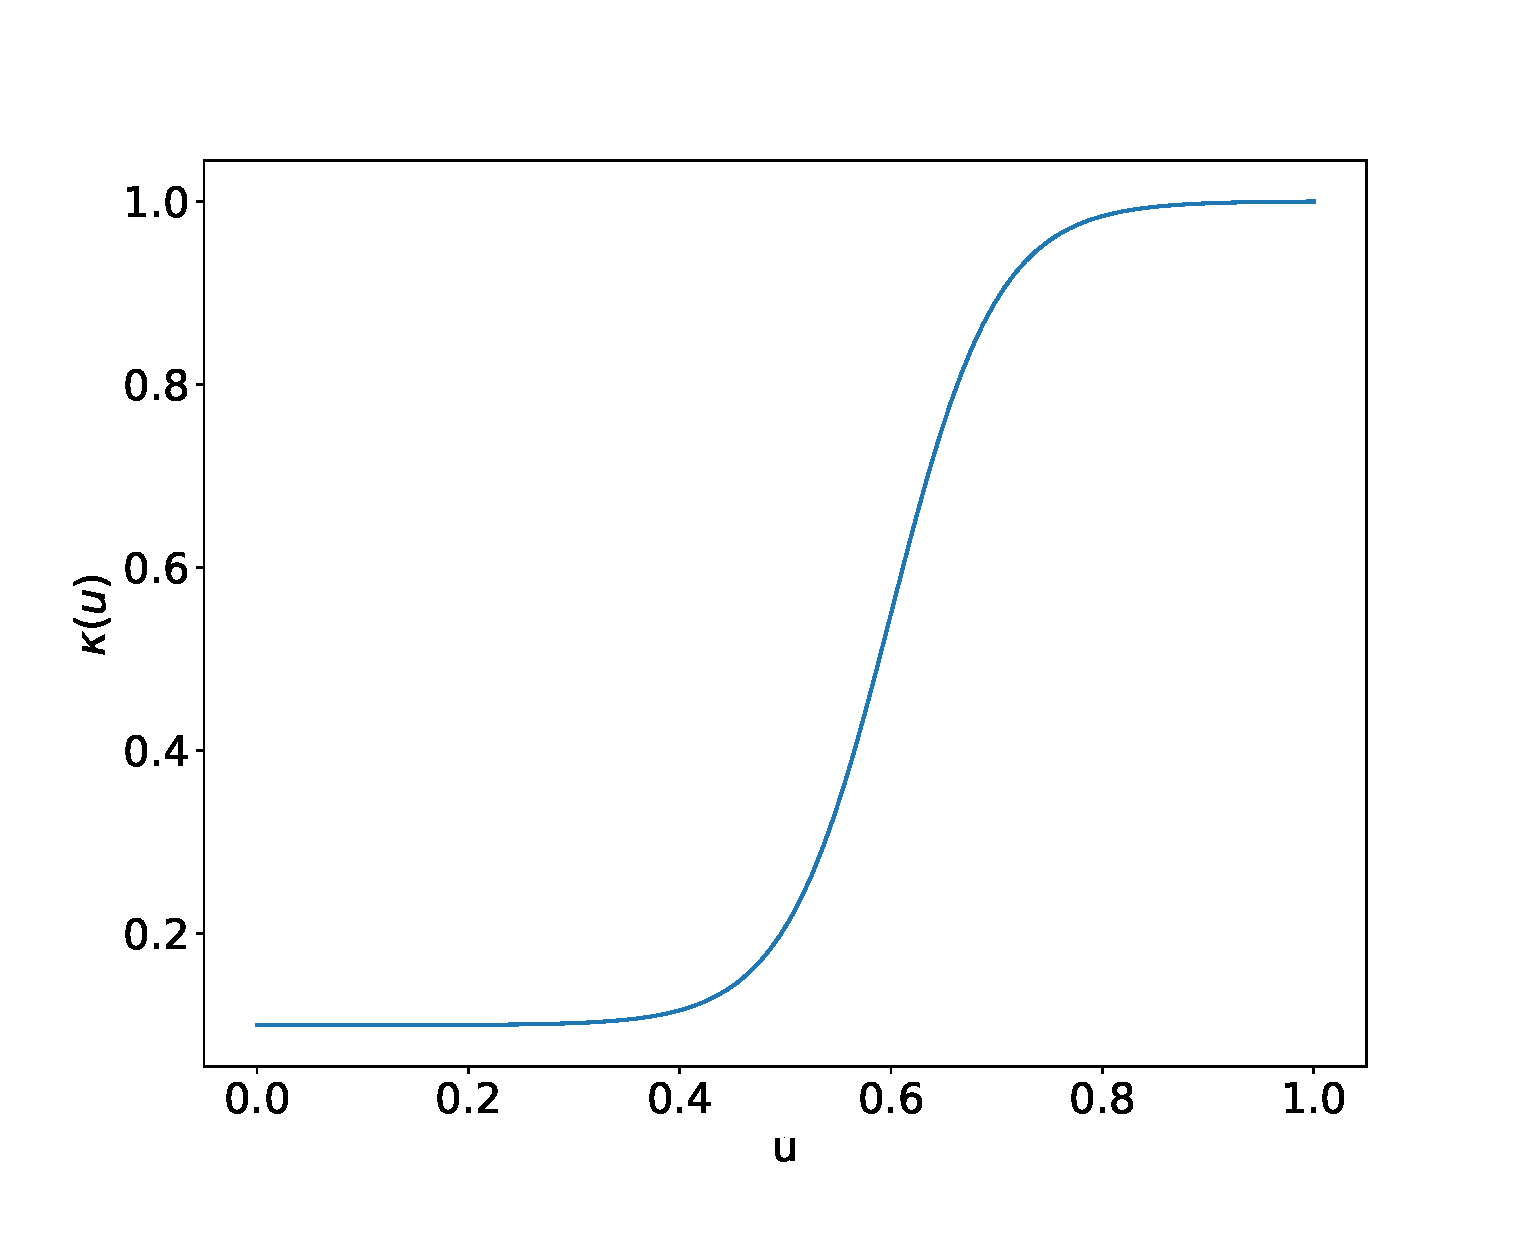
\includegraphics[width=0.5\textwidth]{figures/kappa-u}
					\end{figure}
				\end{multicols}
				
				\vspace{-3em}
        \item Variational Form:
					\[
						F(v, u_n; \Delta t) = \int_\Omega \left(v u_n - \frac{\Delta t}{2} \kappa(u_n) \nabla v \cdot \nabla u\right) \, dx
					\] 
					\[
						A(v, u_{n+1}; \Delta t) = \int_\Omega \left(v u_{n+1} + \frac{\Delta t}{2} \kappa(u_{n+1}) \nabla v \cdot \nabla u_{n+1}\right) \, dx
					\] 
				\end{itemize}
\end{frame}

\begin{frame}{Comparison of Linear and Nonlinear Heat Equations}
	\centering
	\movie[width=10cm,height=6cm, poster]{Comparison Solutions}
	{animations/comparison-heat.avi}
\end{frame}

\begin{frame}{A Nonlinear (Horrible) Example}
    \begin{itemize}
        \item The catenary problem
        
        \begin{equation}
            \min_u \int_{-1}^1 u \sqrt{1 + \left(\epsilon u'\right)^2} \, dx, \quad 
            \text{subject to} \quad 
            \int_{-1}^1 \sqrt{1 + \left(\epsilon u'\right)^2} \, dx = \ell
        \end{equation}
        With $u(\pm 1) = 0$.
        
        \item FEniCS applied to Lagrange Multiplier Problem
        \begin{equation}
            \min_{u, \lambda} \mathcal{F}(u; \lambda) = 
            \int_{-1}^1 u \sqrt{1 + \left(\epsilon u'\right)^2} \, dx - 
            \lambda \int_{-1}^1 \left[\frac{\ell}{2} - \sqrt{1 + \left(\epsilon u'\right)^2}\right] \, dx
        \end{equation}
        
        \item Note $\mathcal F : C^1\left[-1, 1\right] \times \R \to \R$
        
        \item Let $X := C^1\left[-1, 1\right] \times \R$
        
        \item For simplicity, let 
        
        \[
            \der{s}{x} = \sqrt{1 + (\epsilon u')^2}
        \]
    \end{itemize}
\end{frame}


\begin{frame}{Horrible Problem Made Easy}
    \begin{itemize}
        \item Some notation to simplify
        \begin{itemize}
            \item $X:= C^1\left[-1, 1\right] \times \R$ mixed space
            \item $y \in X$, $y = (u, \lambda)$
        \end{itemize}
        \item Minimize $\mathcal F(y) = \mathcal F((u, \lambda)) = \int_{-1}^1 u \der{s}{x} - \lambda \left[\frac{\ell}{2} - 
            \der{s}{x}\right] \, dx$
        \begin{figure}
            \centering
            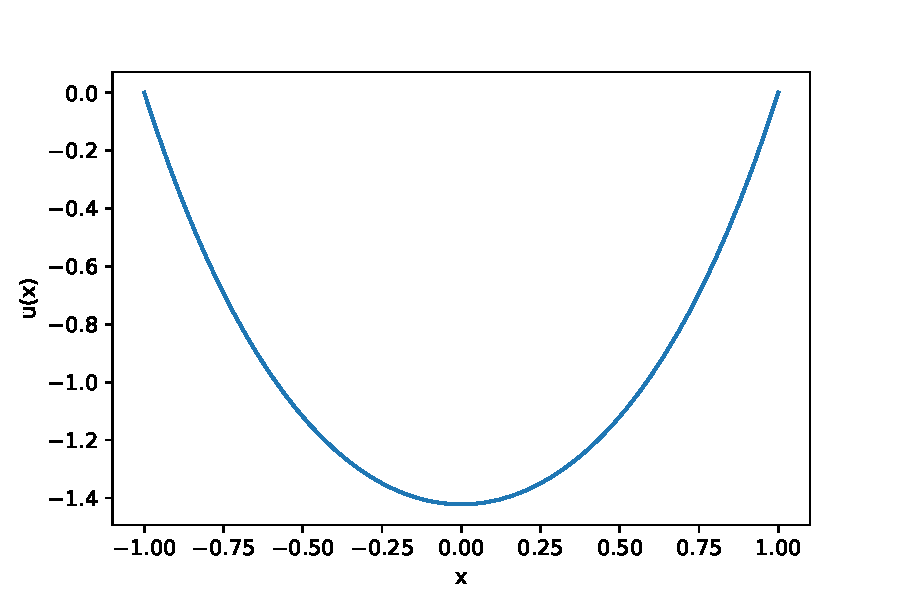
\includegraphics[width=0.65\textwidth,height=0.65\textheight,keepaspectratio]
            {figures/fenics-catenary.pdf}
            \caption{Solution to the Catenary Problem using FEniCS}
            \label{fig:fenics-catenary}
        \end{figure}
    \end{itemize}
\end{frame}

\begin{frame}{Conclusions}
	\begin{itemize}
		\item FEniCS provides an intuitive implementation for finite elements
		\item FEniCS can be overkill for simple problems - it has a lot of overhead
		\item Can solve complicated problems with relative ease
		\item Many more examples on the FEniCS website and book (free)
	\end{itemize}
\end{frame}

\begin{frame}{References}
    \nocite{*}
    \bibliographystyle{plain}
    \bibliography{biblio.bib}
    
    \url{https://github.com/JeromeTroy/fenics-hgss.git}
\end{frame}

\end{document}
